\documentclass[12pt,a4paper]{ufpr}

\usepackage[portuges,brazil]{babel}
% \usepackage[portuguese,brazil]{babel}
%\usepackage[latin1]{inputenc}
%\usepackage{isolatin1}
% \usepackage{auto-pst-pdf}
%\usepackage{epstopdf}
% \usepackage{caption2}
% \usepackage{psfig}

% \usepackage[brazil]{babel}
\usepackage[utf8]{inputenc}
\usepackage[T1]{fontenc}
\usepackage{amssymb,amsmath}
\usepackage{epsfig}
\usepackage{multirow}
\usepackage{ifthen,graphicx,color}
\graphicspath{{img/}}
\usepackage{amssymb}
\usepackage{subfigure}
\usepackage{graphicx}
\usepackage{setspace}
\usepackage{ps-macros}
\usepackage[algochapter,linesnumbered,ruled,inoutnumbered]{algorithm2e}
\usepackage{indentfirst}
\usepackage[hyphens]{url}
\usepackage{hyperref}
\usepackage{csquotes}
\usepackage{listings, lstautogobble}
\usepackage{parcolumns}
\usepackage{subcaption}
\usepackage[dvipsnames]{xcolor}
\usepackage{float}
\usepackage[acronym,nonumberlist,nowarn]{glossaries}
\loadglsentries{0-iniciais/acronimos}

\setcounter{secnumdepth}{3}    % n - numero de niveis de subsubsection numeradas
\setcounter{tocdepth}{3}       % coloca ate o nivel n no sumario

\newcommand{\todo}[1]{{\color{red}\textbf{\ul{?#1}}}}

\lstset{ %
    basicstyle=\linespread{0.9}\ttfamily\scriptsize, % Standardschrift
    language=C,
    numbers=left,               % Ort der Zeilennummern
    numberstyle=\tiny,    % Stil der Zeilennummern
    % ~ numbersep=-15pt,              % Abstand der Nummern zum Text
    tabsize=2,                  % Groesse von Tabs
    % extendedchars=true,         %
    breaklines=true,            % Zeilen werden Umgebrochen
    % breakatwhitespace=true,
    % frame=tb,
    % keywordstyle=\bfseries,
    % stringstyle=\color{white}\ttfamily, % Farbe der Strings
    xleftmargin=12pt,
    % ~ framexleftmargin=0pt,
    % framexrightmargin=-5pt,
    % ~ framexleftmargin=-5pt,
    % framexbottommargin=0pt,
}

\lstdefinelanguage
   [x64]{Assembler}     % add a "x64" dialect of Assembler
   [x86masm]{Assembler} % based on the "x86masm" dialect
   % with these extra keywords:
   {morekeywords={_hmc64_saddimm_d, _hmc64_incr_s, %
                  CDQE,CQO,CMPSQ,CMPXCHG16B,JRCXZ,LODSQ,MOVSXD, %
                  POPFQ,PUSHFQ,SCASQ,STOSQ,IRETQ,RDTSCP,SWAPGS, %
                  rax,rdx,rcx,rbx,rsi,rdi,rsp,rbp, %
                  r8,r8d,r8w,r8b,r9,r9d,r9w,r9b, %
                  r10,r10d,r10w,r10b,r11,r11d,r11w,r11b, %
                  r12,r12d,r12w,r12b,r13,r13d,r13w,r13b, %
                  r14,r14d,r14w,r14b,r15,r15d,r15w,r15b}} % etc.

\lstset{language=[x64]Assembler}

\title{Coligações partidárias no Brasil: Uma análise em grafos}
% \author {Autor do documento}
\autores
{Guilherme Gomes dos Santos}
{Rafael Capaci Pereira}
\advisortitle{Orientador} % ou Orientador
\advisorname{Prof. Dr. André Luis Vignatti}
\advisorplace{Departamento de Informática, UFPR}    % departamento, instituicao
\city{Curitiba}
\year{2017}

\banca  % nao insira o nome do orientador, ja eh feito automaticamente
{Prof. Dr. Nome}{Departamento de Informática, UFPR}
{Prof. Dr. Nome}{Departamento de Informática, UFPR}

\defesa{2017}   % dia em que foi realizada a defesa da dissertacao


\begin{document}

% \makecapaproposta            % cria capa para proposta%
\makecapadissertacao           % cria capa para dissertacao de mestrado %
\makerosto                     % cria folha de rosto para versao final da UFPR %
\maketermo                    % cria folha com o termo de aprovacao da dissertacao%
\pagenumbering{gobble}

%\singlespacing           % espacamento 1 - capa UFPR%
%\onehalfspacing          % espacamento 1/2 %
\doublespacing            % espacamento 2 - UFPR %

\pagestyle{headings}
%\pagenumbering{roman}

% \newpage
% \thispagestyle{empty}
\vspace*{\fill}
\begin{center}
	\textit{obg}
\end{center}
\setcounter{footnote}{0}%

% \chapter*{Agradecimentos}
% thanks    % possiu somente o texto

\newpage
\thispagestyle{empty}
\vspace*{\fill}
\begin{flushright}
	\textit{``Deus é top.``\\
	            Neymar
	 }
\end{flushright}
\setcounter{footnote}{0}%

\pagestyle{headings}

\chapter*{Resumo}
%\addcontentsline{toc}{chapter}{\uppercase{Resumo}}
O presente trabalho  propõe-se a analisar como partidos políticos brasileiros constituem suas alianças na esfera legislativa, para cargos de deputados estaduais. Através da utilização do repositório de dados, obtido no portal do Tribunal Superior Eleitoral (TSE), foram elaborados grafos para cada ano de eleição federal, que, compreende o período dos anos de 1994 à 2014, tal processo surge com o intuito de se avaliar se as coligações partidárias seguem algum padrão político-ideológico. Apresentam-se conceitos necessários para o entendimento do estudo, mostra-se a proposta do trabalho, a metodologia utilizada e em seguida os resultados alcançados. Finaliza-se com uma conclusão geral a respeito dos dados obtidos.



\textbf{Palavras chave:} redes sociais, grafos, política, partidos políticos, coligações.
      % somente o texto
\newpage

\chapter*{Abstract}
%\addcontentsline{toc}{chapter}{\uppercase{Abstract}}
The abstract should be the English translation of the ``resumo'', no more, no less.

\textbf{Keywords:} social networks, graph, politics, brazilian political parties.
    % somente o texto
\newpage

% \listoffigures        % se houver mais do que 3 figuras
% \addcontentsline{toc}{chapter}{\MakeUppercase{Lista de Figuras}}
% \newpage

%\listoftables          % se houver mais do que 3 tabelas
%\addcontentsline{toc}{chapter}{\MakeUppercase{Lista de Tabelas}}

\tableofcontents


% Capítulo 1
\chapter{Introdu{\c   c}{\~a}o}
\label{introducao}
\pagenumbering{arabic}
\setcounter{page}{6} % número da página, sem contar a capa.

%=====================================================

% A introdução geral do documento pode ser apresentada através das seguintes seções: Desafio, Motivação, Proposta, Contribuição e Organização do documento (especificando o que será tratado em cada um dos capítulos). O Capítulo 1 não contém subseções\footnote{Ver o Capítulo \ref{cap-exemplos} para comentários e exemplos de subseções.}.

\begin{comment}Por outro lado, existem também o cenário em que partidos pequenos são ideologicamente consistentes e se unem a partidos com ideais e objetivos em comum. \end{comment}

A formação de alianças é extremamente importante para os partidos políticos brasileiros. Em um sistema altamente fragmentado, unir forças para atingir objetivos eleitorais em comum é a única forma de alguns partidos conseguirem se destacar e obter resultados durante as eleições.

Quando partidos pequenos não possuem representatividade suficiente para disputar um cargo no Executivo, por exemplo, é provável que estes acabem se aliando a um partido maior, em troca de vantagens como cadeiras no Legislativo, cargos em ministérios, secretarias e empresas estatais em caso de uma campanha bem sucedida. Estas alianças - as chamadas \emph{coligações partidárias} - que ocorrem por trocas de favores são altamente prejudiciais para política brasileira, uma vez que se tornam parte de um ciclo vicioso de corrupção entre os partidos. Queremos verificar com este trabalho, utilizando o repositório de dados do TSE e visualizações em grafo, se as coligações são formadas por partidos de afinidade ideológica ou se os interesses políticos acabam se sobressaindo durante a formação das alianças. Fazendo uma análise nos anos de eleição federal compreendidos entre 1994 e 2014, utilizamos um algoritmo de modularidade para a identificação de comunidades nos grafos de coligações para o cargo de deputado estadual.

Este trabalho está organizado da seguinte maneira: No capítulo \ref{conceitos} são apresentados alguns conceitos  sobre teoria de grafos, redes sociais e funcionamentos básicos da política brasileira. No capítulo \ref{proposta} são explicados o objetivo deste estudo e o método utilizada para realizar a análise dos dados afim de atingir os objetivos propostos. No capítulo \ref{resultados} são mostrados os resultados obtidos através de comparativos entre as comunidades identificadas nos grafos e o eixo político dos partidos presentes nas mesmas. Por fim, o capítulo \ref{conclusao} traz uma conclusão geral a respeito do estudo e dos resultados obtidos.


% Capítulo 2
\chapter{Conceitos}
\label{conceitos}

%%%%%%%%%%%%%%%%%%%%%%%%%%%%%%%%%%%%%%%%%%%%%%%%%%%%%%%%%%%
\section{\texorpdfstring{\MakeUppercase{Grafo}}{}}
\label{conceitos__grafo}

Um \emph{grafo} G é um par ordenado (V[G], E[G]) sendo V[G] um conjunto de \emph{vértices} e E[G] um conjunto de \emph{arestas}, onde cada aresta é associada a um par não ordenado de vértices de G através de uma \emph{função de incidência} $\psi_{G}$. Seja \emph{e} uma aresta e \emph{u} e \emph{v} vértices em G, tais que $\psi_{G}$(\emph{e}) = \{\emph{u}, \emph{v}\}, assim, pode-se dizer que \emph{e} é uma aresta que \emph{incide} sobre \emph{u} e \emph{v} e que \emph{u} e \emph{v} são as \emph{extremidades} de \emph{e}. Além disto, é dito que \emph{u} e \emph{v} são vizinhos entre si~\cite{bondy1976graph}.

O número de vértices e arestas em G são denotados por |V[G]| e |E[G]|; estes
dois parâmetros básicos são chamados de \emph{ordem} e \emph{tamanho} de G, respectivamente.

\noindent\emph{Exemplo}.

\makebox[\textwidth]{
    G = (V[G], E[G])
}

\noindent onde

\makebox[\textwidth]{
    V (G) = {u, v, w}
}

\makebox[\textwidth]{
    E(G) = \{e$_{0}$, e$_{1}$\}
}

\noindent e $\psi_{G}$ definida por

\makebox[\textwidth]{
    $\psi_{G}$(\emph{e$_{0}$}) = \{\emph{u}, \emph{v}\}
}

\makebox[\textwidth]{
    $\psi_{G}$(\emph{e$_{1}$}) = \{\emph{v}, \emph{w}\}
}

Visualmente, este grafo pode ser representado da seguinte forma:

\todo{COLOCAR UM DESENHO DA VISUALIZAÇÃO DO GRAFO DO EXEMPLO ANTERIOR}

%%%%%
\subsection{Grau de um vértice}
\label{conceitos__grafo--grau}

\def \variable {\emph{v}}

O \emph{grau} de um vértice \emph{v} em um grafo G, denotado por \emph{d$_{G}$}(\emph{v}), é o número de arestas em G que incidem sobre \emph{v}. De modo particular, \emph{d$_{G}$}(\emph{v}) é o número de vizinhos de \emph{v} em G. Um vértice de grau zero é chamado de \emph{vértice isolado}. O grau mínimo e o grau máximo dos vértices de G são denotados por $\delta(G)$ e $\Delta(G)$, respectivamente, enquanto que \emph{d}(G) denota seu \emph{grau médio}, $\frac{1}{n}\sum_{v\in V}(d(v))$, onde \emph{n} é o número de vértices de G~\cite{bondy1976graph}.

%%%%%

%%%%%
\subsection{Peso}
\label{conceitos__grafo--peso}

Grafos são muito utilizados para modelar problemas reais e, em certos problemas, é preciso incluir alguns atributos especiais, como por exemplo um custo, que está associado com as arestas. Em uma rede de tráfego, por exemplo, esse custo poderia representar a distância entre dois lugares. Esses problemas costumam ser modelados por um grafo ponderado.

Para cada aresta \emph{e} de um grafo G, é associado um número real \emph{w}(\emph{e}), denominado \emph{peso}. Sendo assim, G, com o atributo peso associado as arestas, é chamado de \emph{grafo ponderado}.

%%%%%

\subsection{Componente}
\label{conceitos__grafo--componente}

Um grafo é dito \emph{conexo} se, para cada par de vértices, existe um \emph{caminho} entre eles, ou seja, uma sequência de vértices onde cada par consecutivo na sequência é ligado por uma aresta.

Quando um grafo não é conexo, ele se divide em \emph{componentes}, que são subconjuntos de vértices desse grafo, onde cada par destes vértices possui um caminho entre eles, ou seja, a componente é conexa. Além disso, as componentes são isoladas, ou seja, não existe aresta ligando vértices de diferentes componentes.

\todo{colocar uma figura de um grafo com componentes distintas}

%%%%%
\subsection{Componente Gigante}
\label{conceitos__grafo--componente-gigante}

\emph{Componente gigante} é um termo informal para um componente conexo que contém uma fração significativa de todos os vértices de um grafo.

Além disso, quando um grafo contém um componente gigante, quase sempre este componente é único.

\todo{colocar uma figura de um grafo com uma componente gigante}

%%%%%%%%%%%%%%%%%%%%%%%%%%%%%%%%%%%%%%%%%%%%%%%%%%%%%%%%%%%
\section{\texorpdfstring{\MakeUppercase{Laços Fracos e Fortes}}{}}
\label{conceitos__lacos-fortes-fracos}

Definição de Laços fortes e fracos

%%%%%
\subsection{Fechamento Triádico}
\label{conceitos__lacos-fortes-fracos--fechamento-triadico}

Definição de Fechamento Triádico

%%%%%
\subsection{Coeficiente de clustering}
\label{conceitos__lacos-fortes-fracos--coeficiente-clustering}

Definição de Coeficiente de clustering

%%%%%%%%%%%%%%%%%%%%%%%%%%%%%%%%%%%%%%%%%%%%%%%%%%%%%%%%%%%
\section{\texorpdfstring{\MakeUppercase{Modularidade/comunidades}}{}}
\label{conceitos__modularidade}

Definição de Modularidade/comunidades

%%%%%%%%%%%%%%%%%%%%%%%%%%%%%%%%%%%%%%%%%%%%%%%%%%%%%%%%%%%
\section{\texorpdfstring{\MakeUppercase{Partidos Políticos no Brasil}}{}}
\label{secao_partidos_brasil}

Definição de Partidos Políticos no Brasil

%%%%%%%%%%%%%%%%%%%%%%%%%%%%%%%%%%%%%%%%%%%%%%%%%%%%%%%%%%%

\section{\texorpdfstring{\MakeUppercase{Coligações}}{}}
\label{secao_coligacoes}

Definição de Coligações

\todo{além de definir uma coligação, dizer que no trabalho falamos sobre "um partido fazer coligação com outro" como forma de dizer que "os dois partidos pertencem a uma mesma coligação"}



%%%%%%%%%%%%%%%%%%%%%%%%%%%%%%%%%%%%%%%%%%%%%%%%%%%%%%%%%%%

\section{\texorpdfstring{\MakeUppercase{Espectro Político}}{}}
\label{secao_espectro_politico}

Definição de Espectro Político: Esquerda x Direita

%%%%%%%%%%%%%%%%%%%%%%%%%%%%%%%%%%%%%%%%%%%%%%%%%%%%%%%%%%%

\section{\texorpdfstring{\MakeUppercase{Auto-declaração dos Partidos}}{}}
\label{secao_auto_declaracao_partidos}

Definição de Auto-denominação dos Partidos: (falar que nem todos se auto declaram, mas de certa forma esse seria um dos objetivo deste trabalho. Explicar que os partidos grandes tem a auto declaração)
s
%%%%%%%%%%%%%%%%%%%%%%%%%%%%%%%%%%%%%%%%%%%%%%%%%%%%%%%%%%%

\section{\texorpdfstring{\MakeUppercase{Visualizações}}{}}
\label{secao_visualizacoes}
\subsection{Gephi}
\label{visualizacoes--gephi}

\todo{Explicar sobre o Gephi}

\subsection{Layouts}
\label{visualizacoes--gephi}

\todo{Fazer uma subsection para cada layout do gephi que utilizarmos}


% Capítulo 3
\chapter{Proposta}
\label{cap3_proposta}

%%%%%%%%%%%%%%%%%%%%%%%%%%%%%%%%%%%%%%%%%%%%%%%%%%%%%%%%%%%
\section{\texorpdfstring{\MakeUppercase{Metodologia}}{}}
\label{secao_metodologia}

O site do \gls{TSE} fornece um repositório de dados eleitorais\footnote{\url{http://www.tse.jus.br/eleitor-e-eleicoes/estatisticas/repositorio-de-dados-eleitorais-1}} que contém um compilado de informações brutas das eleições no Brasil, sendo assim um meio para pesquisadores, imprensa e pessoas interessadas analisarem dados de candidatura, eleitorado, resultados e prestação de contas. Estes dados são fornecidos em arquivos no formato \emph{.csv}, de forma que consultas, filtros e cruzamento de dados são de responsabilidade do pesquisador.

Além dos arquivos, o site do \gls{TSE} fornece uma documentação que visa explicar como os dados estão dispostos em cada tipo de arquivo. Após estudo da documentação fornecida, elaboramos um modelo relacional dos dados para possibilitar um melhor entendimento do conteúdo disponível e decidir quais informações seriam interessantes para análise. Nesta etapa percebeu-se que existiam arquivos com dados incompletos e formatações diferentes na disposição de seus conteúdos, gerando assim uma redução de dados que poderiam ser analisados forma satisfatória.

Esta inconsistência encontrada em alguns dados nos levou a desistir de uma ideia inicial, na qual pretendia-se analisar as coligações para eleições presidenciais. Dessa forma, optou-se por focar o estudo nas coligações formadas para disputa ao cargo de deputado estadual.

Dentre os arquivos estudados, avaliou-se que os dados referentes aos candidatos eram os mais completos, apresentando inclusive informações sobre partidos e coligações. Dessa forma, optamos por observar o relacionamento entre os partidos políticos ao longo dos anos de eleição.

\todo{explicar o parser}

A próxima etapa foi realizar o tratamento destes dados brutos, afim de extrair somente os dados que eram do interesse deste trabalho. Para isso, foi escrito um programa em linguagem \emph{Javascript}, que recebe como entrada os arquivos de dados, um arquivo com o esquema dos dados, ou seja, a informação de quais são os campos do tipo de arquivo que está sendo lido e o cargo político de interesse para a análise.

Este programa então converte estes dados para o formato \emph{JSON}\footnote{\emph{Javascript Object Notation}: formato de padrão aberto utilizado para transmitir objetos de dados consistindo de pares chave-valor.}, que é o formato utilizado em \emph{Javascript} para representar objetos em memória em tempo de execução. Este formato e as facilidades da linguagem permitem que seja realizado um filtro dos dados, de maneira rápida e prática. Após a filtragem dos dados, trabalhamos em moldá-los em uma estrutura de grafos, ainda no formato \emph{JSON}. Por fim, são gerados os arquivos de saída em formato \emph{.gexf}\footnote{Formato padrão do \emph{Gephi}, muito similar ao formato \emph{.xml}, mas com algumas particularidades. Especificação do formato \emph{.gexf} disponível em: \url{https://gephi.org/gexf/format}.}. São gerados vários arquivos de saída, sendo um para cada ano de eleição. Este programa está disponível, de maneira aberta e gratuita, em \url{https://github.com/xurupito/tg-parser}

\todo{revisar...}
%%%%%%%%%%%%%%%%%%%%%%%%%%%%%%%%%%%%%%%%%%%%%%%%%%%%%%%%%%%
\section{\texorpdfstring{\MakeUppercase{Modelagem}}{}}
\label{subsecao_modelagem}

Após a obtenção dos dados formatados da maneira desejada, foi definido que seriam analisadas coligações partidárias estaduais em âmbito nacional, para o cargo de deputado. Duas possíveis abordagens para a modelagem em grafos surgiram:
\begin{itemize}
    \item Gerar um grafo por estado. Cada partido político seria um vértice e os partidos que participassem de uma mesma coligação seriam conectados por uma aresta.
    \item Gerar um grafo ponderado por ano. Cada vértice seria um partido e as arestas conectariam partidos de mesmas coligações. O peso das arestas representaria em quantos estados os dois partidos participam de uma mesma coligação naquele ano.
\end{itemize}

Avaliou-se exemplos de grafos dentro do primeiro cenário, e percebeu-se que em cada estado o grafo correspondente apresentava diversas cliques, cada uma sendo uma coligação.

\begin{figure}[H]
\centering
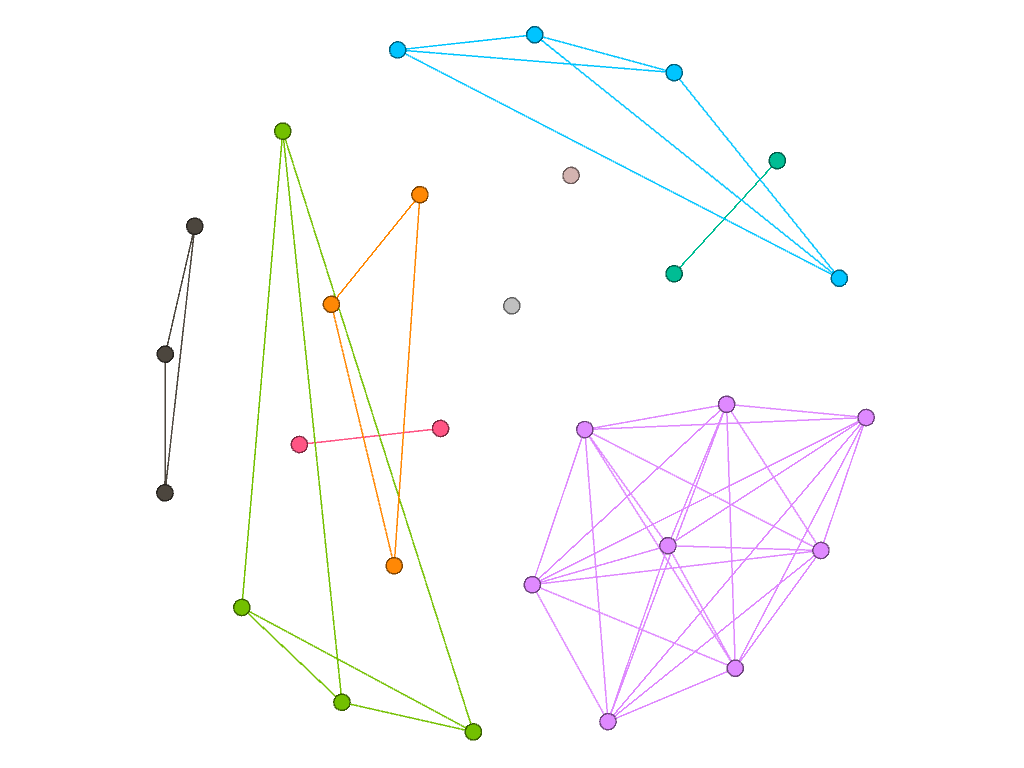
\includegraphics[width=1\textwidth]{img/parana-1998.png}
\caption{Grafo de coligações do Paraná em 1998.}
\end{figure}

Percebemos que esta modelagem não seria proveitosa, pois exigiria uma grande quantidade de grafos e mesmo assim não seria possível obter as informações desejadas para este trabalho. Desta forma, adotamos a segunda abordagem.

%%%%%%%%%%%%%%%%%%%%%%%%%%%%%%%%%%%%%%%%%%%%%%%%%%%%%%%%%%%
\section{\texorpdfstring{\MakeUppercase{Restrições}}{}}
\label{secao_objetivo_geral}

A divisão ideológica dos partidos no Brasil não é trivial, no atual sistema político existem siglas com programas vagos e ideologias pouco claras, o que dificulta sua categorização dentro do espectro político. Com isso tornou-se inviável a categorização de alguns partidos presentes nos grafos apresentados neste trabalho.

Não é difícil perceber que existe falta de consenso dentro do cenário político como um todo em relação a como partidos se posicionam ou se encaixam no espectro político brasileiro, e essa categorização é inclusive foco de estudo de historiadores e sociólogos. Dessa forma, para a classificação dos partidos em \emph{esquerda}, \emph{direita}, \emph{centro} e as demais divisões ideológicas, optamos por dar prioridade a como os partidos se auto declaram (quando o fazem). Nos demais casos, categorizamos de acordo com classificações encontradas em \todo{referencias}.

Por fim, entendemos que foge da proposta deste trabalho discorrer sobre questões socio-políticas a respeito dos dados apresentados, uma vez que estas questões podem ser melhor discutidas por estudiosos de outras áreas do conhecimento, como sociólogos, historiadores e cientistas políticos.

%%%%%%%%%%%%%%%%%%%%%%%%%%%%%%%%%%%%%%%%%%%%%%%%%%%%%%%%%%%
\section{\texorpdfstring{\MakeUppercase{Revisão da Bibliografia}}{}}
\label{secao_revisao_bibliografia}

Algo light. Algum trabalho que possa ter motivado o nosso


%%%%%

%%%%%%%%%%%%%%%%%%%%%%%%%%%%%%%%%%%%%%%%%%%%%%%%%%%%%%%%%%%
\section{\texorpdfstring{\MakeUppercase{Objetivo Geral}}{}}
\label{secao_objetivo_geral}

\todo{Talvez seja interessante apresentar algum contexto mais político, falar de informações interessantes q encontramos sei la}
Este trabalho propõe-se a utilizar o repositório de dados do \gls{TSE} para a construção de grafos referentes às informações de coligações partidárias no Brasil nos anos 1994 à 2014, com o objetivo de exibir métricas e visualizações que possam indicar se as coligações são formadas por partidos de ideologias semelhantes.

%%%%%%%%%%%%%%%%%%%%%%%%%%%%%%%%%%%%%%%%%%%%%%%%%%%%%%%%%%%
\section{\texorpdfstring{\MakeUppercase{Objetivos Específicos}}{}}
\label{secao_objetivos_especificos}

%% Objetivos Específicos: ("pontual", em formato de lista. São pequenos objetivos para chegar/alcançar o objetivo geral do trabalho)
\subsection{Categorização dos partidos dentro do espectro político brasileiro}
\label{subsecao_modularizacao}

Avaliar os dados obtidos no repositório do \gls{TSE} é categorizar todos os partidos encontrados como sendo de esquerda, centro-esquerda, centro, centro-direita e direita. Esta categorização é feita inteiramente baseando-se nas informações apresentadas pelas referências utilizadas neste trabalho.

A classificação dos partidos dentro do espectro político nos permite entender quais partidos - em teoria - possuem afinidades ideológicas, gerando assim um meio de criarmos um referencial de como partidos se relacionariam se eles seguissem suas ideologias como base para criar coligações.

\subsection{Identificação de comunidades}
\label{subsecao_modularizacao}

Apresentar grafos para os anos de eleição estadual - 1994, 1998, 2002, 2006, 2010 e 2014 - e aplicar o algoritmo de modularização disponível no Gephi para a identificação de comunidades nestes grafos. Utilizando a categorização dos partidos dentro do espectro político, podemos analisar se as comunidades encontradas seguem algum padrão ideológico.

Optamos por tentar manter os grafos com duas comunidades, o que nos permite identificar se existe alguma divisão entre partidos de esquerda e direita.

\subsection{Análise e comparação dos grafos gerados}
\label{subsecao_modularizacao}

Utilizar a classificação de espectro político para analisar e comparar qual o padrão ideológico dos partidos presentes nas comunidades encontradas. Isso é feito através da geração de um segundo grafo para cada ano, no qual cada vértice é colorido de acordo com seu espectro político. Vértices em tom de vermelho são partidos de centro-esquerda, esquerda e extrema-esquerda. Vértices em tom de azul são partidos de centro-direita, direita e extrema-direita. Já os vértices verdes são os partidos que se declaram de centro, e os em tom cinza são os partidos que não foi possível classificar dentro do espectro político.

Esta abordagem provê uma facilidade na análise das comunidades, já que é possível comparar os grafos lado a lado e identificar relacionamentos entre os partidos, tamanho das comunidades, ideologia politica predonominante em cada agrupamento de vértices etc.
%%%%%
\subsection{Informações apresentadas}
\label{subsecao_infos_apresentadas}

qual é o interesse em apresentar as informações sobre grau médio, coeficiente de clustering, ...

% Capítulo 3
\chapter{Proposta}
\label{proposta}

%%%%%%%%%%%%%%%%%%%%%%%%%%%%%%%%%%%%%%%%%%%%%%%%%%%%%%%%%%%
\section{\texorpdfstring{\MakeUppercase{Metodologia}}{}}
\label{proposta__metodologia}

O site do \gls{TSE} fornece um repositório de dados eleitorais\footnote{\url{http://www.tse.jus.br/eleitor-e-eleicoes/estatisticas/repositorio-de-dados-eleitorais-1}} que contém um compilado de informações brutas das eleições no Brasil, sendo assim um meio para pesquisadores, imprensa e pessoas interessadas analisarem dados de candidatura, eleitorado, resultados e prestação de contas. Estes dados são fornecidos em arquivos no formato \emph{.csv}, de forma que consultas, filtros e cruzamento de dados são de responsabilidade do pesquisador.

Além dos arquivos, o site do \gls{TSE} fornece uma documentação que visa explicar como os dados estão dispostos em cada tipo de arquivo. Após estudo da documentação fornecida, elaboramos um modelo relacional dos dados para possibilitar um melhor entendimento do conteúdo disponível e decidir quais informações seriam interessantes para análise. Nesta etapa percebeu-se que existiam arquivos com dados incompletos e formatações diferentes na disposição de seus conteúdos, gerando assim uma redução de dados que poderiam ser analisados forma satisfatória.

Esta inconsistência encontrada em alguns dados nos levou a desistir de uma ideia inicial, na qual pretendia-se analisar as coligações para eleições presidenciais. Dessa forma, optou-se por focar o estudo nas coligações formadas para disputa ao cargo de deputado estadual.

Dentre os arquivos estudados, avaliou-se que os dados referentes aos candidatos eram os mais completos, apresentando inclusive informações sobre partidos e coligações. Dessa forma, optamos por observar o relacionamento entre os partidos políticos ao longo dos anos de eleição.

\todo{explicar o parser}

A próxima etapa foi realizar o tratamento destes dados brutos, afim de extrair somente os dados que eram do interesse deste trabalho. Para isso, foi escrito um programa em linguagem \emph{Javascript}, que recebe como entrada os arquivos de dados, um arquivo com o esquema dos dados, ou seja, a informação de quais são os campos do tipo de arquivo que está sendo lido e o cargo político de interesse para a análise.

Este programa então converte estes dados para o formato \emph{JSON}\footnote{\emph{Javascript Object Notation}: formato de padrão aberto utilizado para transmitir objetos de dados consistindo de pares chave-valor.}, que é o formato utilizado em \emph{Javascript} para representar objetos em memória em tempo de execução. Este formato e as facilidades da linguagem permitem que seja realizado um filtro dos dados, de maneira rápida e prática. Após a filtragem dos dados, trabalhamos em moldá-los em uma estrutura de grafos, ainda no formato \emph{JSON}. Por fim, são gerados os arquivos de saída em formato \emph{.gexf}\footnote{Formato padrão do \emph{Gephi}, muito similar ao formato \emph{.xml}, mas com algumas particularidades. Especificação do formato \emph{.gexf} disponível em: \url{https://gephi.org/gexf/format}.}. São gerados vários arquivos de saída, sendo um para cada ano de eleição. Este programa está disponível, de maneira aberta e gratuita, em \url{https://github.com/xurupito/tg-parser}.

\todo{revisar...}
%%%%%%%%%%%%%%%%%%%%%%%%%%%%%%%%%%%%%%%%%%%%%%%%%%%%%%%%%%%
\section{\texorpdfstring{\MakeUppercase{Modelagem}}{}}
\label{proposta__modelagem}

Após a obtenção dos dados formatados da maneira desejada, foi definido que seriam analisadas coligações partidárias estaduais em âmbito nacional, para o cargo de deputado. Duas possíveis abordagens para a modelagem em grafos surgiram:
\begin{itemize}
    \item Gerar um grafo por estado. Cada partido político seria um vértice e os partidos que participassem de uma mesma coligação seriam conectados por uma aresta.
    \item Gerar um grafo ponderado por ano. Cada vértice seria um partido e as arestas conectariam partidos de mesmas coligações. O peso das arestas representaria em quantos estados os dois partidos participam de uma mesma coligação naquele ano.
\end{itemize}

Avaliou-se exemplos de grafos dentro do primeiro cenário, e percebeu-se que em cada estado o grafo correspondente apresentava diversas cliques, cada uma sendo uma coligação.

\begin{figure}[H]
\centering
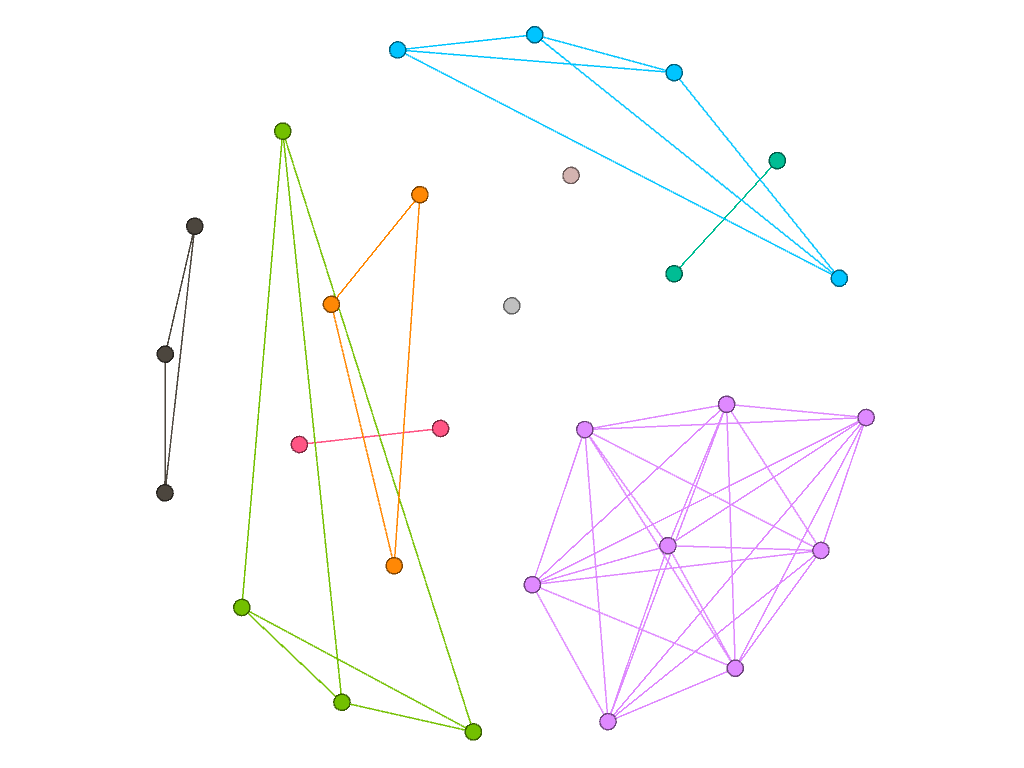
\includegraphics[width=1\textwidth]{img/parana-1998.png}
\caption{Grafo de coligações do Paraná em 1998.}
\end{figure}

Percebemos que esta modelagem não seria proveitosa, pois exigiria uma grande quantidade de grafos e mesmo assim não seria possível obter as informações desejadas para este trabalho. Desta forma, adotamos a segunda abordagem.

%%%%%%%%%%%%%%%%%%%%%%%%%%%%%%%%%%%%%%%%%%%%%%%%%%%%%%%%%%%
\section{\texorpdfstring{\MakeUppercase{Restrições}}{}}
\label{proposta__restricoes}

A divisão ideológica dos partidos no Brasil não é trivial, no atual sistema político existem siglas com programas vagos e ideologias pouco claras, o que dificulta sua categorização dentro do espectro político. Com isso tornou-se inviável a categorização de alguns partidos presentes nos grafos apresentados neste trabalho.

Não é difícil perceber que existe falta de consenso dentro do cenário político como um todo em relação a como partidos se posicionam ou se encaixam no espectro político brasileiro, e essa categorização é inclusive foco de estudo de historiadores e sociólogos. Dessa forma, para a classificação dos partidos em \emph{esquerda}, \emph{direita}, \emph{centro} e as demais divisões ideológicas, optamos por dar prioridade a como os partidos se auto declaram (quando o fazem). Nos demais casos, categorizamos de acordo com classificações encontradas em \todo{referencias}.

Por fim, entendemos que foge da proposta deste trabalho discorrer sobre questões socio-políticas a respeito dos dados apresentados, uma vez que estas questões podem ser melhor discutidas por estudiosos de outras áreas do conhecimento, como sociólogos, historiadores e cientistas políticos.

%%%%%%%%%%%%%%%%%%%%%%%%%%%%%%%%%%%%%%%%%%%%%%%%%%%%%%%%%%%
\section{\texorpdfstring{\MakeUppercase{Revisão da Bibliografia}}{}}
\label{proposta__revisao_bibliografia}

Algo light. Algum trabalho que possa ter motivado o nosso


%%%%%

%%%%%%%%%%%%%%%%%%%%%%%%%%%%%%%%%%%%%%%%%%%%%%%%%%%%%%%%%%%
\section{\texorpdfstring{\MakeUppercase{Objetivo Geral}}{}}
\label{proposta__objetivo-geral}

\todo{Talvez seja interessante apresentar algum contexto mais político, falar de informações interessantes q encontramos sei la}
Este trabalho propõe-se a utilizar o repositório de dados do \gls{TSE} para a construção de grafos referentes às informações de coligações partidárias no Brasil nos anos 1994 à 2014, com o objetivo de exibir métricas e visualizações que possam indicar se as coligações são formadas por partidos de ideologias semelhantes.

%%%%%%%%%%%%%%%%%%%%%%%%%%%%%%%%%%%%%%%%%%%%%%%%%%%%%%%%%%%
\section{\texorpdfstring{\MakeUppercase{Objetivos Específicos}}{}}
\label{proposta__objetivos-especificos}

%% Objetivos Específicos: ("pontual", em formato de lista. São pequenos objetivos para chegar/alcançar o objetivo geral do trabalho)
\subsection{Categorização dos partidos dentro do espectro político brasileiro}
\label{proposta__objetivos-especificos--categorizacao}

Avaliar os dados obtidos no repositório do \gls{TSE} é categorizar todos os partidos encontrados como sendo de esquerda, centro-esquerda, centro, centro-direita e direita. Esta categorização é feita inteiramente baseando-se nas informações apresentadas pelas referências utilizadas neste trabalho.

A classificação dos partidos dentro do espectro político nos permite entender quais partidos - em teoria - possuem afinidades ideológicas, gerando assim um meio de criarmos um referencial de como partidos se relacionariam se eles seguissem suas ideologias como base para criar coligações.

\subsection{Identificação de comunidades}
\label{proposta__objetivos-especificos--identificacao-comunidades}

Apresentar grafos para os anos de eleição estadual - 1994, 1998, 2002, 2006, 2010 e 2014 - e aplicar o algoritmo de modularização disponível no Gephi para a identificação de comunidades nestes grafos. Utilizando a categorização dos partidos dentro do espectro político, podemos analisar se as comunidades encontradas seguem algum padrão ideológico.

Optamos por tentar manter os grafos com duas comunidades, o que nos permite identificar se existe alguma divisão entre partidos de esquerda e direita.

\subsection{Análise e comparação dos grafos gerados}
\label{proposta__objetivos-especificos--analise-comparacao}

Utilizar a classificação de espectro político para analisar e comparar qual o padrão ideológico dos partidos presentes nas comunidades encontradas. Isso é feito através da geração de um segundo grafo para cada ano, no qual cada vértice é colorido de acordo com seu espectro político. Vértices em tom de vermelho são partidos de centro-esquerda, esquerda e extrema-esquerda. Vértices em tom de azul são partidos de centro-direita, direita e extrema-direita. Já os vértices verdes são os partidos que se declaram de centro, e os em tom cinza são os partidos que não foi possível classificar dentro do espectro político.

Esta abordagem provê uma facilidade na análise das comunidades, já que é possível comparar os grafos lado a lado e identificar relacionamentos entre os partidos, tamanho das comunidades, ideologia politica predonominante em cada agrupamento de vértices etc.
%%%%%
\subsection{Informações apresentadas}
\label{proposta__objetivos-especificos--informacoes-apresentadas}

qual é o interesse em apresentar as informações sobre grau médio, coeficiente de clustering, ...

% Capítulo 2
\chapter{Conclusão e trabalhos futuros}
\label{conclusao}

\todo{Acho que podemos detalhar um pouco mais este primeiro parágrafo, citando algumas métricas encontradas? }

Utilizando os conhecimentos em computação adquiridos durante a graduação, especialmente em teoria de grafos e redes sociais, foi possível analisar como se comportaram as coligações partidárias no Brasil no período entre 1994 e 2014. Constatou-se que embora os partidos formassem um número maior de alianças com aqueles de ideologias políticas similares, esta distinção tornou-se menos evidente nos anos subsequentes. O número de alianças entre diferentes legendas cresceu consideravelmente, enquanto a quantidade de partidos no país não teve uma mudança significativa.

Um dos maiores desafios encontrados durante o desenvolvimento deste trabalho foi utilizar o repositório no site do \gls{TSE}. Arquivos com formatações inconsistentes, conteúdos incompletos e uma carência por filtros e modelagem adequada dos dados dificultam a utilização de informações que são fundamentais para estudos sobre a política brasileira. Com isso, esperamos conseguir elaborar um meio mais eficiente de utilizar os dados do repositório, através da criação de uma modelagem relacional e uma \emph{API}, podendo assim,  viabilizar e incentivar mais estudos a cerca destes dados e fornecer uma maneira simples do público em geral ter conhecimento sobre os mesmos.




%\input{anexo1.tex}     % se houver anexo



% utilize macros (3 primeiras letras do mes em ingles, minusculas) no seu
% .bib para atribuir o nome do mes em portugues nas referencia,
% se o style for brazil, outros estilos tambem aceitam estas macros
% Ex:
%
% @InProceedings{teste,
%   author =       {Luciano}
%   year =         {2000}
%   month =        {}#sep;
% }
%


\bibliographystyle{apalike}
\bibliography{99-final/bibliografia}
\addcontentsline{toc}{chapter}{REFERÊNCIAS}


\singlespacing
% \makecapadissertacao

\end{document}
